\chapter{Fonaments}

\section{Introducci\'{o}}
Es tracten en aquest cap\'{\i}tol q\"{u}estions b\`{a}siques
d'electrot\`{e}cnia, com ara teoremes, definicions i relacions.


\section{Teoremes d'electrot\`{e}cnia}\label{sec:teoremes}

\subsection{\texorpdfstring{Teorema de Th\'{e}venin--Norton}{Teorema de
            Th\'{e}venin-Norton}}\label{sec:T_N}

\index{teorema!de Th\'{e}venin}El teorema de Th\'{e}venin ens permet
substituir una xarxa complexa formada per elements lineals, per un
circuit equivalent format per una font de tensi\'{o} $\cmplx{E}\ped{Th}$
en s\`{e}rie amb una imped\`{a}ncia $\cmplx{Z}\ped{Th}$.


Atenent a la Figura \vref{pic:Thevenin}, si coneixem la tensi\'{o} en
buit $\cmplx{U}\ped{o}$ entre dos nusos $\alphaup$ i $\betaup$ d'una
xarxa, i la imped\`{a}ncia $\cmplx{Z}_{\alphaup\betaup}$ d'aquesta xarxa
vista des d'aquests dos nusos, podem obtenir els valors del circuit
Th\'{e}venin equivalent entre aquests dos nusos, a partir de les
relacions seg\"{u}ents:\index{ETh@$E\ped{Th}$}\index{ZTh@$Z\ped{Th}$}
\begin{equation}
   \cmplx{E}\ped{Th} = \cmplx{U}\ped{o} \qquad\qquad  \cmplx{Z}\ped{Th} = \cmplx{Z}_{\alphaup\betaup}
\end{equation}

D'aquesta manera, la connexi\'{o} d'aquesta xarxa a trav\'{e}s dels nusos
$\alphaup$ i $\betaup$ a una c\`{a}rrega qualsevol $\cmplx{Z}\ped{Q}$, \'{e}s
equivalent pel que fa a aquesta c\`{a}rrega, a connectar el circuit
equivalent Th\'{e}venin a la c\`{a}rrega.
\begin{center}
    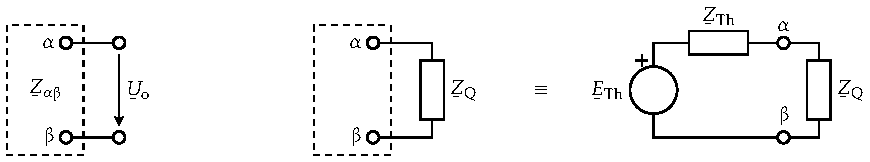
\includegraphics{Imatges/Cap-Fonaments-Thevenin.pdf}
    \captionof{figure}{Teorema de Th\'{e}venin}
    \label{pic:Thevenin}
\end{center}

\index{teorema!de Norton}El teorema de Norton ens permet substituir
una xarxa complexa formada per elements lineals, per un circuit
equivalent format per una font de corrent $\cmplx{J}\ped{No}$ en
para{\l.l}el amb una admit\`{a}ncia $\cmplx{Y}\ped{No}$.

Atenent a la Figura \vref{pic:Norton}, si coneixem el corrent de
curtcircuit $\cmplx{I}\ped{cc}$ entre dos nusos $\alphaup$ i $\betaup$
d'una xarxa, i l'admit\`{a}ncia $\cmplx{Y}_{\alphaup\betaup}$ d'aquesta
xarxa vista des d'aquests dos nusos, podem obtenir els valors del
circuit Norton equivalent entre aquests dos nusos, a partir de les
relacions seg\"{u}ents:\index{JNo@$J\ped{No}$}\index{YNo@$Y\ped{No}$}
\begin{equation}
   \cmplx{J}\ped{No} = \cmplx{I}\ped{cc} \qquad\qquad \cmplx{Y}\ped{No} = \cmplx{Y}_{\alphaup\betaup}
\end{equation}

D'aquesta manera, la connexi\'{o} d'aquesta xarxa a trav\'{e}s dels nusos
$\alphaup$ i $\betaup$ a una c\`{a}rrega qualsevol $\cmplx{Z}\ped{Q}$, \'{e}s
equivalent pel que fa a aquesta c\`{a}rrega, a connectar el circuit
equivalent Norton a la c\`{a}rrega.
\begin{center}
    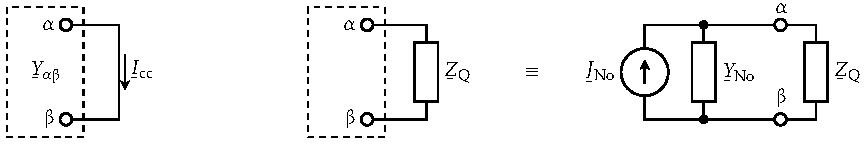
\includegraphics{Imatges/Cap-Fonaments-Norton.pdf}
    \captionof{figure}{Teorema de Norton}
    \label{pic:Norton}
\end{center}

Els circuits Th\'{e}venin i Norton d'una xarxa s\'{o}n equivalents entre si.
Els par\`{a}metres que defineixen aquests circuits compleixen les relacions
seg\"{u}ents:
\begin{equation}\label{eq:Thevenin-Norton}
   \cmplx{E}\ped{Th} = \frac{\cmplx{J}\ped{No}}{\cmplx{Y}\ped{No}} \qquad\qquad
   \cmplx{J}\ped{No} = \frac{\cmplx{E}\ped{Th}}{\cmplx{Z}\ped{Th}} \qquad\qquad
    \cmplx{Z}\ped{Th} = \frac{1}{\cmplx{Y}\ped{No}}
\end{equation}

Els valors $\cmplx{Z}\ped{Th}$ i  $\cmplx{Y}\ped{No}$ es poden
obtenir substituint en la xarxa  les fonts de tensi\'{o}  per curtcircuits, i les fonts de corrent per circuits oberts, i calculant
aleshores la imped\`{a}ncia o admit\`{a}ncia equivalent\footnote{El c\`{a}lcul sistem\`{a}tic de $\cmplx{Z}\ped{Th}$ i  $\cmplx{Y}\ped{No}$ en una xarxa qualsevol, s'exposa en la secci\'{o} \ref{sec:xarxes_Zth}}.

\subsection{Teorema de Millman}\label{sec:millman}

\index{teorema!de Millman}Atenent a la Figura \vref{pic:Millman}, el teorema
de Millman ens permet
obtenir la tensi\'{o} de l'extrem com\'{u} $\nuup$ de diverses imped\`{a}ncies respecte d'un punt
qualsevol $\alphaup$, a partir de les tensions dels altres extrems de les imped\`{a}ncies respecte
 del mateix punt $\alphaup$.

\hfill
\begin{minipage}[b]{7cm}
    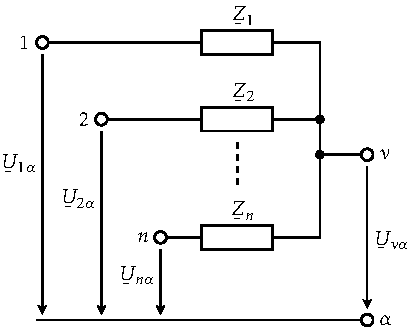
\includegraphics{Imatges/Cap-Fonaments-Millman.pdf}
    \captionof{figure}{Teorema de Millman}
    \label{pic:Millman}
\end{minipage}
\hfill
\begin{minipage}[b][4.5cm][t]{6cm}
    \begin{equation}
        \cmplx{U}_{\nuup\alphaup} = \frac{\displaystyle\sum_{k=1}^n \dfrac{\cmplx{U}_{k\alphaup}}{\cmplx{Z}_k}} {\displaystyle\sum_{k=1}^n \dfrac{1}{\cmplx{Z}_k}}
    \end{equation}
\end{minipage}


\pagebreak

\begin{exemple}[Aplicaci\'{o} del Teorema de Millman]
    A partir de la figura seg\"{u}ent, es tracta de determinar els circuits
    Th\'{e}venin i Norton equivalents del circuit format per les tres
    bateries i les seves resist\`{e}ncies, i calcular la tensi\'{o} i el
    corrent que existirien en una resist\`{e}ncia de c\`{a}rrega
    $R\ped{Q}=\SI{50}{\ohm}$, que es connect\'{e}s entre els punts $\alphaup$
    i $\nuup$.

    \begin{center}
        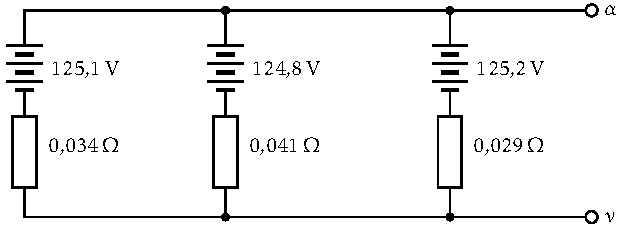
\includegraphics{Imatges/Cap-Fonaments-Millman-Exemple1.pdf}
    \end{center}

    La imped\`{a}ncia Th\'{e}venin equivalent es calcula, tal com s'ha dit en la Secci\'{o} \ref{sec:T_N},
    substituint en el circuit totes les fonts de tensi\'{o} per curtcircuits; aix\'{\i} doncs, ens
    queden tres resist\`{e}ncies en para{\l.l}el entre $\alphaup$ i $\nuup$:
    \[
    Z\ped{Th} = \frac{1}{\dfrac{1}{\SI{0,034}{\ohm}} +
    \dfrac{1}{\SI{0,041}{\ohm}} + \dfrac{1}{\SI{0,029}{\ohm}}} =
    \SI{0,01133}{\ohm}
    \]

    Per calcular la font de tensi\'{o} Th\'{e}venin equivalent, utilitzarem el
    teorema de Millman. Si es compara aquest circuit amb el de la Figura
    \vref{pic:Millman}, veiem que els punts $\alphaup$ i $\nuup$ dels dos
    circuits s\'{o}n equivalents, \'{e}s a dir, $\nuup$ \'{e}s el punt com\'{u} de les
    imped\`{a}ncies, i $\alphaup$ \'{e}s el punt de refer\`{e}ncia dels altres extrems
    de les imped\`{a}ncies, respecte del qual les tensions s\'{o}n conegudes
    (tensions de les bateries). Aix\'{\i} doncs tenim:
    \[
    U_{\nuup\alphaup} = \frac{\dfrac{\SI{-125,1}{V}}{\SI{0,034}{\ohm}} +
    \dfrac{\SI{-124,8}{V}}{\SI{0,041}{\ohm}} +
    \dfrac{\SI{-125,2}{V}}{\SI{0,029}{\ohm}}}{\dfrac{1}{\SI{0,034}{\ohm}}
    + \dfrac{1}{\SI{0,041}{\ohm}} + \dfrac{1}{\SI{0,029}{\ohm}}} =
    \SI{-125,0562}{V}
    \]

    La font de tensi\'{o}  Th\'{e}venin equivalent entre $\alphaup$ i $\nuup$ \'{e}s per
    tant:
    \[
    E\ped{Th} = U_{\alphaup\nuup} = \SI{125,0562}{V}
    \]

    Calculem a continuaci\'{o} l'admit\`{a}ncia i la font de corrent  Norton equivalents, utilitzant
    l'equaci\'{o} \eqref{eq:Thevenin-Norton}:
    \begin{align*}
        Y\ped{No} &= \frac{1}{Z\ped{Th}} = \frac{1}{\SI{0,01133}{\ohm}} = \SI{82,2613}{S}
        \\[2ex]
        J\ped{No} &= \frac{E\ped{Th}}{Z\ped{Th}} =
        \frac{\SI{125,0562}{V}}{\SI{0,01133}{\ohm}}= \SI{11037,6150}{A}
    \end{align*}

    Tal com s'ha dit en la Secci\'{o} \ref{sec:T_N}, J\ped{No} \'{e}s igual al
    corrent de curtcircuit entre els punts $\alphaup$ i $\nuup$.

    Finalment, ja podem calcular el corrent $I\ped{Q}$ i la tensi\'{o} $U\ped{Q}$ en la
    resist\`{e}ncia de c\`{a}rrega, utilitzant el circuit Th\'{e}venin equivalent calculat anteriorment:
    \begin{align*}
        I\ped{Q} &= \frac{E\ped{Th}}{Z\ped{Th} + R\ped{Q}} = \frac{\SI{125,0562}{V}}
        {\SI{0,01133}{\ohm} + \SI{50}{\ohm}} = \SI{2,5001}{A} \\[2ex]
        U\ped{Q} &=  R\ped{Q} \,I\ped{Q} = \SI{50}{\ohm} \times \SI{2,5001}{A} =
        \SI{125,0050}{V}
    \end{align*}
\end{exemple}


\begin{exemple}[Aplicaci\'{o} del Teorema de Millman]
    Tenim un generador trif\`{a}sic connectat en estrella, amb una tensi\'{o} fase--neutre de \SI{230}{V}; el punt neutre de l'estrella est\`{a} connectat a terra a traves d'una resist\`{e}ncia de \SI{46}{\ohm}. El generador alimenta tres c\`{a}rregues resistives connectades entre cadascuna de les fases i terra de valors \SI{50}{m\ohm}, \SI{80}{m\ohm} i \SI{70}{m\ohm} respectivament. Es tracta de trobar el corrent que circula per la resist\`{e}ncia de connexi\'{o} a terra del generador, i els que circulen per cadascuna de les tres c\`{a}rregues.

    En el dibuix seg\"{u}ent es pot veure el circuit el\`{e}ctric que es vol resoldre.

    \begin{center}
        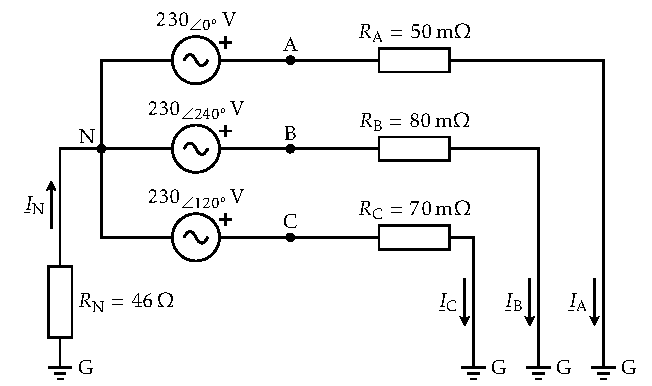
\includegraphics{Imatges/Cap-Fonaments-Millman-Exemple2.pdf}
    \end{center}

    La tensi\'{o} $\cmplx{U}\ped{GN}$ es pot calcular directament aplicant el teorema de Millman. Per fer-ho, nom\'{e}s cal tenir en compte que les quatre resist\`{e}ncies del circuit tenen un punt com\'{u} que \'{e}s {"<}G{">}, i que les tensions dels altres extrems de les resist\`{e}ncies respecte del punt {"<}N{">} s\'{o}n conegudes: $\cmplx{U}\ped{AN}=\SIpd{230}{0}{V}$, $\cmplx{U}\ped{BN}=\SIpd{230}{240}{V}$, $\cmplx{U}\ped{CN}=\SIpd{230}{120}{V}$ i  $\cmplx{U}\ped{NN}=\SI{0}{V}$.

    Aix\'{\i} doncs tenim:
    \[
    \cmplx{U}\ped{GN} = \frac{ \dfrac{\cmplx{U}\ped{AN}}{R\ped{A}} + \dfrac{\cmplx{U}\ped{BN}}{R\ped{B}} + \dfrac{\cmplx{U}\ped{CN}}{R\ped{C}} + \dfrac{\cmplx{U}\ped{NN}}{R\ped{N}}} { \dfrac{1}{R\ped{A}} + \dfrac{1}{R\ped{B}} + \dfrac{1}{R\ped{C}} + \dfrac{1}{R\ped{N}} } =
    \frac{\dfrac{\SIpd{230}{0}{V}}{\SI{50}{m\ohm}}+\dfrac{\SIpd{230}{240}{V}}{\SI{80}{m\ohm}}+
    \dfrac{\SIpd{230}{120}{V}}{\SI{70}{m\ohm}}}{\dfrac{1}{\SI{50}{m\ohm}}+\dfrac{1}{\SI{80}{m\ohm}}+
    \dfrac{1}{\SI{70}{m\ohm}}+\dfrac{1}{\SI{46}{\ohm}}} =
    \SIpd{33,34}{13,17}{V}
    \]

    El corrent  que circula per la resist\`{e}ncia de connexi\'{o} a terra del generador val:
    \[
    \cmplx{I}\ped{N} = \frac{\cmplx{U}\ped{GN}}{R\ped{N}} = \frac{\SIpd{33,34}{13,17}{V}}{\SI{46}{\ohm}}
    = \SIpd{725}{13,17}{mA}
    \]

    Finalment, els corrents que circulen per cadascuna de les tres c\`{a}rregues val:
    \begin{align*}
    \cmplx{I}\ped{A} &= \frac{\cmplx{U}\ped{AG}}{R\ped{A}} = \frac{\cmplx{U}\ped{AN} + \cmplx{U}\ped{NG}}{R\ped{A}} = \frac{\SIpd{230}{0}{V}-\SIpd{33,34}{13,17}{V}}{\SI{50}{m\ohm}}
    = \SIpd{3,954}{-2,20}{kA}\\[2ex]
    \cmplx{I}\ped{B} &= \frac{\cmplx{U}\ped{BG}}{R\ped{B}} = \frac{\cmplx{U}\ped{BN} + \cmplx{U}\ped{NG}}{R\ped{B}} = \frac{\SIpd{230}{240}{V}-\SIpd{33,34}{13,17}{V}}{\SI{80}{m\ohm}}
    = \SIpd{3,175}{234,51}{kA}\\[2ex]
    \cmplx{I}\ped{C} &= \frac{\cmplx{U}\ped{CG}}{R\ped{C}} = \frac{\cmplx{U}\ped{CN} + \cmplx{U}\ped{NG}}{R\ped{C}} = \frac{\SIpd{230}{120}{V}-\SIpd{33,34}{13,17}{V}}{\SI{70}{m\ohm}}
    = \SIpd{3,454}{127,59}{kA}
    \end{align*}
\end{exemple}


\subsection{Teorema de la superposici\'{o}}\index{teorema!de la
superposici\'{o}}

Si tenim un circuit lineal on hi ha diverses fonts de tensi\'{o} i  de
corrent, les quals originen corrents i caigudes de tensi\'{o} en els
components del circuit, el teorema de la superposici\'{o} ens diu que
podem calcular aquests corrents i caigudes de tensi\'{o}, resolent els
circuits que resulten de tenir en compte  nom\'{e}s una font de tensi\'{o} o
de corrent a l'hora, i sumant al final els valors parcials
obtinguts.

En cada pas on considerem nom\'{e}s una font de tensi\'{o} o de corrent, hem
d'eliminar la resta de fonts del circuit; per tal de fer-ho hem de
substituir la resta de fonts de tensi\'{o} per un curtcircuit, i la
resta de fonts de corrent per un circuit obert.

Aquest teorema tamb\'{e} \'{e}s aplicable en el cas que tinguem nom\'{e}s una
font de tensi\'{o} o de corrent, que operi a m\'{e}s d'una freq\"{u}\`{e}ncia a
l'hora. En aquest cas es pot estudiar el circuit de forma
independent per a cadascuna de les freq\"{u}\`{e}ncies presents, i sumar al
final els valors parcials obtinguts.

\begin{exemple}[Aplicaci\'{o} del teorema de la superposici\'{o}]
    Es tracta de trobar en el circuit seg\"{u}ent, el corrent $\cmplx{I}$ que circula
    pel condensador, utilitzant el teorema de la superposici\'{o}.
    \begin{center}
        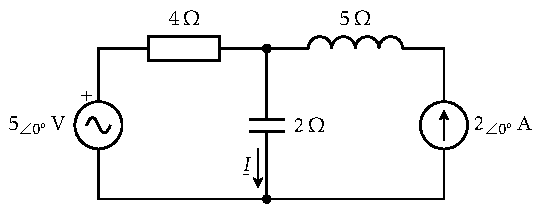
\includegraphics{Imatges/Cap-Fonaments-Exemple-Superposicio-1.pdf}
    \end{center}

    Utilitzant el teorema de la superposici\'{o}, representem els dos
    circuits seg\"{u}ents a partir del circuit original. El circuit de
    l'esquerra nom\'{e}s t\'{e} la font de tensi\'{o}, amb la font de corrent
    substitu\"{\i}da per un circuit obert, i el circuit de
    la dreta nom\'{e}s t\'{e} la font de corrent, amb la font de tensi\'{o}
    substitu\"{\i}da per un curtcircuit.
    \begin{center}
        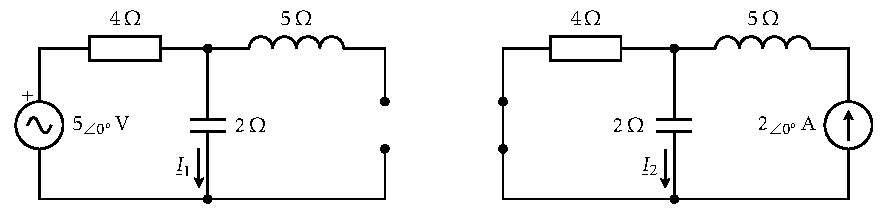
\includegraphics{Imatges/Cap-Fonaments-Exemple-Superposicio-2.pdf}
    \end{center}

    Els corrents $\cmplx{I}_1$ i $\cmplx{I}_2$ que circulen pel condensador valen:
    \[
        \cmplx{I}_1 = \frac{\SIpd{5}{0}{V}}{\SI{4-2j}{\ohm}} =
        \SIpd{1,118}{26,57}{A} \qquad\qquad
        \cmplx{I}_2 = \frac{\dfrac{1}{\frac{1}{\SI{4}{\ohm}}+\frac{1}{\SI{-2j}{ \ohm}}}}
        {\SI{-2j}{ \ohm}} \times \SIpd{2}{0}{A} = \SIpd{1,789}{26,57}{A}
    \]

    El corrent total $\cmplx{I}$ que circula pel condensador val:
    \[
        \cmplx{I}  = \cmplx{I}_1 + \cmplx{I}_2 = \SIpd{1,118}{26,57}{A} +  \SIpd{1,789}{26,57}{A} =
        \SIpd{2,907}{26,57}{A}
    \]
\end{exemple}



\section{Valors mitj\`{a} i efica\c{c}, i factors de cresta, de forma i
d'arrissada}\label{sec:val_mitja_ef}

S'explica a continuaci\'{o} com obtenir diversos par\`{a}metres caracter\'{\i}stics de funcions peri\`{o}diques  en el temps $v(t)$, de freq\"{u}\`{e}ncia $f$, per\'{\i}ode $T$ i velocitat angular $\omega$; les relacions que compleixen aquests tres par\`{a}metres s\'{o}n: $f = 1/T$ i $\omega=2\piup f = 2\piup\,/T$.

Les funcions peri\`{o}diques poden  definir-se en funci\'{o} de l'angle $\alpha$, enlloc del temps $t$; es compleixen les relacions:
$\alpha=\omega t$ i $\diff\alpha=\omega\diff t$.

\subsection{Valor mitj\`{a}}\index{valor!mitj\`{a}}

El valor mitj\`{a} $\bar{V}$ d'una funci\'{o}
peri\`{o}dica en el temps $v(t)$ es
defineix com\footnote{En la Secci\'{o} \ref{sec:four_val_av} es defineix el valor mitj\`{a} d'una funci\'{o} peri\`{o}dica expressada en s\`{e}ries de Fourier.}:
\begin{equation}
    \bar{V} = \frac{1}{T} \int_{t_0}^{t_0+T} v(t) \diff t =
    \frac{\omega}{2\piup} \int_{t_0}^{t_0+\frac{2\piup}{\omega}} v(t) \diff t\label{eq:vm_t}
\end{equation}

Si la funci\'{o} peri\`{o}dica $v(\alpha)$ est\`{a} definida en funci\'{o} de
l'angle $\alpha$, enlloc del temps $t$, tenim:
\begin{equation}
    \bar{V} = \frac{1}{2\piup} \int_{\alpha_0}^{\alpha_0+2\piup} v(\alpha) \diff \alpha
    \label{eq:vm_alfa}
\end{equation}

\subsection{Valor efica\c{c}}\index{valor!efica\c{c}}
\index{root mean square@\guillemotleft root mean
square\guillemotright}\index{rms}

El valor efica\c{c}  $V$ (tamb\'{e} anomenat valor rms, de l'angl\`{e}s {"<}root
mean square{">}) d'una funci\'{o} peri\`{o}dica en el temps $v(t)$ es defineix com\footnote{En la Secci\'{o} \ref{sec:four_val_ef} es defineix el valor efica\c{c} d'una funci\'{o} peri\`{o}dica expressada en s\`{e}ries de Fourier.}:
\begin{equation}
    V = \sqrt{\frac{1}{T} \int_{t_0}^{t_0+T} [v(t)]^2 \diff
    t} = \sqrt{\frac{\omega}{2\piup} \int_{t_0}^{t_0+\frac{2\piup}{\omega}}
     [v(t)]^2 \diff t}
\end{equation}

Si la funci\'{o} peri\`{o}dica $v(\alpha)$ est\`{a} definida en funci\'{o} de
l'angle $\alpha$, enlloc del temps $t$, tenim:
\begin{equation}
    V = \sqrt{\frac{1}{2\piup} \int_{\alpha_0}^{\alpha_0+2\piup}
     [v(\alpha)]^2 \diff \alpha}
\end{equation}

\subsection{Factor de cresta}
\index{factor!de cresta}

El factor de cresta relaciona els valors de cresta $\hat{V}$
  i efica\c{c} $V$ d'una funci\'{o} peri\`{o}dica. La norma \textsf{CEI 60050} l'anomena {"<}peak factor{">} i el defineix com:\index{CEI!60050-00@60050}
\begin{equation}
     \frac{\hat{V}}{V}
\end{equation}

\subsection{Factor de forma}\index{factor!de forma}\index{F@$F$}

El factor de forma relaciona els valors efica\c{c} $V$
i mitj\`{a} $\bar{V}$ d'una funci\'{o} peri\`{o}dica. La norma \textsf{CEI 60050} l'anomena {"<}form factor{">}, li assigna el s\'{\i}mbol $F$ i el defineix com:\index{CEI!60050-00@60050}
\begin{equation}
    F = \frac{V}{|\bar{V}|}
\end{equation}

\subsection{Factor d'arrissada efica\c{c}}\index{factor!d'arrissada efica\c{c}}\index{r@$r$}

El factor d'arrissada efica\c{c} relaciona els
valors mitj\`{a} $\bar{V}$ i efica\c{c} $V$ d'una funci\'{o} peri\`{o}dica.
La norma \textsf{CEI 60050} l'anomena {"<}rms-ripple factor{">} o {"<}relative ripple content{">}, li assigna el s\'{\i}mbol $r$ i el defineix com\footnote{En la Secci\'{o} \ref{sec:four_fac_arr_ef} es defineix el factor d'arrissada efica\c{c} d'una funci\'{o} peri\`{o}dica expressada en s\`{e}ries de Fourier.}:\index{CEI!60050-00@60050}
\begin{equation}
    r = \sqrt{\frac{V^2}{\bar{V}^2}-1} = \sqrt{F^2-1}\label{eq:rms_rip}
\end{equation}

Aquest factor s'utilitza usualment per definir la qualitat d'una
tensi\'{o} continua, rectificada a partir d'una tensi\'{o} alterna; com m\'{e}s
plana sigui aquesta tensi\'{o} cont\'{\i}nua m\'{e}s baix ser\`{a} el seu factor
d'arrissada.

\subsection{Factor d'arrissada de cresta}\index{factor!d'arrissada de cresta}\index{q@$q$}

El factor d'arrissada de cresta relaciona els valors de cresta $\hat{V}$, de vall $\check{V}$  i mitj\`{a} $\bar{V}$
 d'una funci\'{o} peri\`{o}dica. La norma \textsf{CEI 60050} l'anomena {"<}peak-ripple factor{">} o {"<}peak distortion{">}, li assigna el s\'{\i}mbol $q$ i el defineix com:\index{CEI!60050-00@60050}
\begin{equation}
    q = \frac{\hat{V} - \check{V}}{|\bar{V}|}
\end{equation}

\begin{exemple}[C\`{a}lcul de factors de cresta, de forma i d'arrissada]
    Es tracta de calcular els factors de cresta, de forma i d'arrissada
    de la tensi\'{o}  que s'obt\'{e}, a partir d'una tensi\'{o} sinuso\"{\i}dal
    $u(t) = \hat{U} \sin\omega t$, amb un rectificador de mitja ona i
    amb un rectificador d'ona completa.

    En el cas del rectificador de mitja ona, la tensi\'{o} que s'obt\'{e} ve
    definida per:
    \[
    u(t) = \begin{cases} \hat{U} \sin\omega t, & 0 < \omega t < \piup\\
           0, & \piup \leq \omega t \leq 2\piup \end{cases}
    \]

    Calculem en primer lloc el valor mitj\`{a}:
    \[
    \bar{U} = \frac{\omega}{2\piup} \left( \int_0^\frac{\piup}{\omega}
    \hat{U} \sin\omega t \diff t +
    \int_\frac{\piup}{\omega}^\frac{2\piup}{\omega} 0 \diff t \right) = -
    \left. \frac{\hat{U} \cos\omega t}{2\piup}
    \right|_0^\frac{\piup}{\omega} = \frac{\hat{U}}{\piup}
    \]

    Calculem a continuaci\'{o} el valor efica\c{c}:
    \[
    U = \sqrt{\frac{\omega}{2\piup} \left( \int_0^\frac{\piup}{\omega}
    \hat{U}^2 \sin^2\omega t \diff t +
    \int_\frac{\piup}{\omega}^\frac{2\piup}{\omega} 0 \diff t \right)} =
      \sqrt{\left.\frac{\omega \hat{U}^2}{2\piup}\left( \frac{t}{2} -
    \frac{\sin (2\omega t)}{4\omega}
    \right)\right|_0^\frac{\piup}{\omega}} = \frac{\hat{U}}{2}
    \]

    Els factors de cresta, de forma i d'arrissada s\'{o}n:
    \begin{align*}
        \text{factor de cresta} &= \frac{\hat{U}}{\hat{U}/2} = 2 \\[0.5ex]
        F &= \frac{\hat{U}/2}{\hat{U}/\piup} =\frac{\piup}{2} =
        \num{1,57} \\[0.5ex]
        r &= \sqrt{\left(\frac{\hat{U}/2}{\hat{U}/\piup}\right)^2-1} =
    \sqrt{\frac{\piup^2}{4}-1} = \num{1,21} \\[0.5ex]
        q &= \frac{\hat{U} - 0}{\hat{U}/\piup} = \piup = \num{3,14}
    \end{align*}


    En el cas del rectificador d'ona completa, la tensi\'{o} que s'obt\'{e} ve
    definida per:
    \[
    u(t) = \begin{cases} \phantom{-}\hat{U} \sin\omega t, & 0 < \omega t < \piup\\
           -\hat{U} \sin\omega t, & \piup \leq \omega t \leq 2\piup \end{cases}
    \]

    En aquest cas, l'ona de tensi\'{o} entre $\piup$ i $2\piup$ \'{e}s una repetici\'{o}
    exacta de l'ona de tensi\'{o} entre 0 i $\piup$, per tant, \'{u}nicament
    caldr\`{a} considerar-ne la primera meitat (entre 0 i $\piup$), tenint en
    compte que el per\'{\i}ode ser\`{a} $\piup\,/\omega$.

     Calculem en primer lloc el valor mitj\`{a}:
    \[
    \bar{U} = \frac{\omega}{\piup} \int_0^\frac{\piup}{\omega} \hat{U}
    \sin\omega t \diff t  = - \left. \frac{\hat{U} \cos\omega t}{\piup}
    \right|_0^\frac{\piup}{\omega} = \frac{2 \hat{U}}{\piup}
    \]

    Calculem a continuaci\'{o} el valor efica\c{c}:
    \[
    U = \sqrt{\frac{\omega}{\piup} \int_0^\frac{\piup}{\omega} \hat{U}^2
    \sin^2\omega t \diff t } =   \sqrt{\left.\frac{\omega
    \hat{U}^2}{\piup}\left( \frac{t}{2} - \frac{\sin (2\omega t)}{4\omega}
    \right)\right|_0^\frac{\piup}{\omega}}  = \frac{\hat{U}}{\sqrt{2}}
    \]

    Els factors de cresta, de forma i d'arrissada s\'{o}n:
    \begin{align*}
        \text{factor de cresta} &= \frac{\hat{U}}{\hat{U}/\sqrt{2}} = \sqrt{2} \\[0.5ex]
        F &= \frac{\hat{U}/\sqrt{2}}{2 \hat{U}/\piup} =\frac{\piup}{2\sqrt{2}} =
        \num{1,11} \\[0.5ex]
    r &= \sqrt{\left(\frac{\hat{U}/\sqrt{2}}{2 \hat{U}/\piup}\right)^2-1}
    = \sqrt{\frac{\piup^2}{8}-1} = \num{0,48}\\[0.5ex]
    q &=  \frac{\hat{U} - 0}{2 \hat{U}/\piup} = \frac{\piup}{2} = \num{1,57}
    \end{align*}
\end{exemple}

\section{Pot\`{e}ncia complexa}\label{sec:pot_complex} \index{pot\`{e}ncia complexa}

\subsection{Pot\`{e}ncia monof\`{a}sica} \index{pot\`{e}ncia complexa!monof\`{a}sica}

En la Figura \vref{pic:pot_comp_mono} es representa una c\`{a}rrega $\cmplx{Z}=R+\ju X$, la
qual absorbeix una pot\`{e}ncia complexa $\cmplx{S} = P + \ju Q$.
\begin{center}
    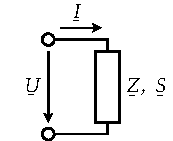
\includegraphics{Imatges/Cap-Fonaments-Potencia-Monof.pdf}
    \captionof{figure}{Pot\`{e}ncia complexa monof\`{a}sica}
    \label{pic:pot_comp_mono}
\end{center}

$R$ i $X$ s\'{o}n respectivament la part resistiva i la part reactiva
(inductiva o capacitiva) de la c\`{a}rrega, i $P$ i $Q$ s\'{o}n
respectivament la potencia activa i la potencia reactiva (inductiva
o capacitiva) absorbida per la c\`{a}rrega.

La pot\`{e}ncia activa absorbida per una c\`{a}rrega sempre \'{e}s positiva, en
canvi, la pot\`{e}ncia reactiva absorbida per una c\`{a}rrega pot ser
positiva o negativa, segons que predomini m\'{e}s la part inductiva o la
part capacitiva de la c\`{a}rrega respectivament.

L'angle $\varphiup$ entre els fasors $\cmplx{U}$ i $\cmplx{I}$ compleix la seg\"{u}ent relaci\'{o}:
\begin{equation}
   \tan\varphiup = \frac{X}{R} = \frac{Q}{P}
\end{equation}

\index{factor!de pot\`{e}ncia}A partir d'aquest angle $\varphiup$, es
defineix el factor de pot\`{e}ncia de la c\`{a}rrega:
\begin{equation}
   \text{Factor de pot\`{e}ncia} \equiv \cos\varphiup
\end{equation}

At\`{e}s que per a un angle qualsevol $\alphaup$ es compleix la igualtat
trigonom\`{e}trica: $\cos\alphaup = \cos(-\alphaup)$, quan es d\'{o}na el factor
de pot\`{e}ncia d'una c\`{a}rrega, cal especificar si \'{e}s inductiu ($Q>0,
\tan\varphiup>0$) o capacitiu ($Q<0, \tan\varphiup<0$); aix\`{o} es fa
afegint {"<}(i){">} o {"<}(c){">} respectivament al valor num\`{e}ric del factor
de pot\`{e}ncia, com per exemple: $\cos\varphiup=0,8$(i),
$\cos\varphiup=0,9$(c).

Les relacions que lliguen la pot\`{e}ncia complexa amb la tensi\'{o} i el corrent s\'{o}n:
\begin{align}
   \cmplx{S} &=  \cmplx{U} \,\cmplx{I}^* =
   |\cmplx{I}|^2 \,\cmplx{Z} = \frac{|\cmplx{U}|^2}{\cmplx{Z}^*} =
   P + \ju Q \label{eq:s_mono1}\\
   |\cmplx{S}| &= |\cmplx{U}| \,|\cmplx{I}| =
   |\cmplx{I}|^2 \,|\cmplx{Z}| = \frac{|\cmplx{U}|^2}{|\cmplx{Z}|} =
   \sqrt{P^2+Q^2} \\
   P &= \Re (\cmplx{U} \, \cmplx{I}^*) = |\cmplx{S}| \cos\varphiup =
   |\cmplx{U}|\, |\cmplx{I}| \cos\varphiup = |\cmplx{I}|^2 R =
   \frac{|\cmplx{U}|^2}{|\cmplx{Z}|^2}R\\
   Q &= \Im (\cmplx{U} \, \cmplx{I}^*) = |\cmplx{S}| \sin\varphiup =
   |\cmplx{U}| \,|\cmplx{I}|\sin\varphiup  = |\cmplx{I}|^2 X =
   \frac{|\cmplx{U}|^2}{|\cmplx{Z}|^2}X
\end{align}

\subsection{Pot\`{e}ncia trif\`{a}sica} \index{pot\`{e}ncia complexa!trif\`{a}sica}

En la Figura \vref{pic:pot_comp_trif} es representen dos sistemes
d'alimentaci\'{o} a c\`{a}rregues trif\`{a}siques; el de l'esquerra \'{e}s un
sistema de 4 fils (3 fases + neutre) i el de la dreta \'{e}s un sistema
de 3 fils (3 fases). En ambd\'{o}s casos es consideren tres c\`{a}rregues
$\cmplx{Z}_\alphaup = R_\alphaup + \ju X_\alphaup$, $\cmplx{Z}_\betaup=
R_\betaup + \ju X_\betaup$ i $\cmplx{Z}_\gammaup= R_\gammaup + \ju X_\gammaup$
connectades en estrella, les quals absorbeixen respectivament unes
pot\`{e}ncies complexes $\cmplx{S}_\alphaup= P_\alphaup + \ju Q_\alphaup$,
$\cmplx{S}_\betaup= P_\betaup + \ju Q_\betaup$ i $\cmplx{S}_\gammaup=
P_\gammaup + \ju Q_\gammaup$.

$R_\alphaup$, $R_\betaup$ i $R_\gammaup$, i $X_\alphaup$, $X_\betaup$ i
$X_\gammaup$ s\'{o}n respectivament les parts resistives i les parts
reactives (inductives o capacitives) de les c\`{a}rregues, i $P_\alphaup$,
$P_\betaup$ i $P_\gammaup$, i $Q_\alphaup$, $Q_\betaup$ i $Q_\gammaup$ s\'{o}n
respectivament les potencies actives i les potencies reactives
(inductives o capacitives) absorbides per les c\`{a}rregues.

El sistema d'alimentaci\'{o} de 3 fils, admet tamb\'{e} c\`{a}rregues
trif\`{a}siques connectades en triangle; en aquest cas nom\'{e}s cal dur a
terme la transformaci\'{o} a una connexi\'{o} en estrella (vegeu la Secci\'{o}
\ref{secc:d_y}), i per tant, la descripci\'{o} que segueix es pot
considerar del tot general.

\begin{center}
    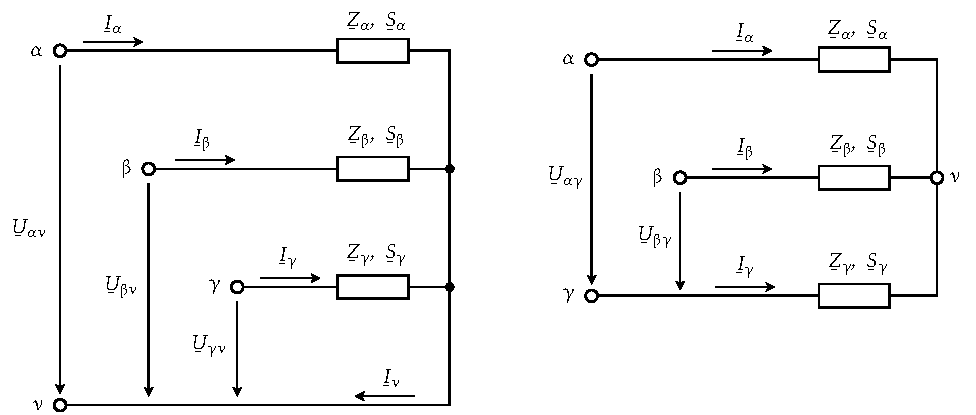
\includegraphics{Imatges/Cap-Fonaments-Potencia-Trif.pdf}
    \captionof{figure}{Pot\`{e}ncia complexa trif\`{a}sica. Sistemes de 4 fils i 3 fils respectivament.}
    \label{pic:pot_comp_trif}
\end{center}

En el cas m\'{e}s general, on la c\`{a}rrega trif\`{a}sica \'{e}s desequilibrada,
cada imped\`{a}ncia t\'{e} el seu propi factor de pot\`{e}ncia
$\cos\varphiup_\alphaup$, $\cos\varphiup_\betaup$ i $\cos\varphiup_\gammaup$,
complint-se:
\begin{equation}
    \tan\varphiup_\alphaup = \frac{X_\alphaup}{R_\alphaup} = \frac{Q_\alphaup}{P_\alphaup} \qquad
    \tan\varphiup_\betaup = \frac{X_\betaup}{R_\betaup} = \frac{Q_\betaup}{P_\betaup} \qquad
    \tan\varphiup_\gammaup = \frac{X_\gammaup}{R_\gammaup} = \frac{Q_\gammaup}{P_\gammaup}
\end{equation}

\subsubsection{Sistema equilibrat o desequilibrat (de 3 fils o de 4 fils)}

Aquest \'{e}s el cas m\'{e}s general, ja que les tensions, la c\`{a}rrega o
ambdues a l'hora  poden ser desequilibrades, i el sistema
d'alimentaci\'{o} pot ser de 3 fils o de 4 fils.

En el cas del sistema d'alimentaci\'{o} de 4 fils tenim:
$\cmplx{I}_\alphaup+\cmplx{I}_\betaup+\cmplx{I}_\gammaup=\cmplx{I}_\nuup$, i
en el cas del sistema d'alimentaci\'{o} de 3 fils tenim:
$\cmplx{I}_\alphaup+\cmplx{I}_\betaup+\cmplx{I}_\gammaup=0$. No obstant,
si prenem en ambd\'{o}s casos el punt $\nuup$ com a refer\`{e}ncia de les
tensions, el corrent $\cmplx{I}_\nuup$ no intervindr\`{a} en el c\`{a}lcul de
la pot\`{e}ncia. Aix\'{\i} doncs, les relacions que lliguen la pot\`{e}ncia
complexa trif\`{a}sica $\cmplx{S}\ped{3F} = P\ped{3F} + \ju Q\ped{3F}$
amb les tensions i corrents s\'{o}n:

\begin{align}
    \cmplx{S}\ped{3F} &= \cmplx{S}_\alphaup + \cmplx{S}_\betaup + \cmplx{S}_\gammaup =
     \cmplx{U}_{\alphaup\nuup}\, \cmplx{I}_\alphaup^* +
    \cmplx{U}_{\betaup\nuup} \,\cmplx{I}_\betaup^* +  \cmplx{U}_{\gammaup\nuup}\, \cmplx{I}_\gammaup^* =
    (P_\alphaup + P_\betaup + P_\gammaup) + \ju (Q_\alphaup + Q_\betaup + Q_\gammaup) \label{eq:s_3f} \\
    |\cmplx{S}\ped{3F}| &= |\cmplx{S}_\alphaup + \cmplx{S}_\betaup + \cmplx{S}_\gammaup| =
    |\cmplx{U}_{\alphaup\nuup}\, \cmplx{I}_\alphaup^* +
    \cmplx{U}_{\betaup\nuup}\, \cmplx{I}_\betaup^* +  \cmplx{U}_{\gammaup\nuup} \,\cmplx{I}_\gammaup^*| =
    \sqrt{(P_\alphaup + P_\betaup + P_\gammaup)^2 + (Q_\alphaup + Q_\betaup + Q_\gammaup)^2} \label{eq:s_3f_mod} \\
    P\ped{3F} &= \Re(\cmplx{U}_{\alphaup\nuup} \,\cmplx{I}_\alphaup^*) +
    \Re(\cmplx{U}_{\betaup\nuup} \,\cmplx{I}_\betaup^*) +  \Re(\cmplx{U}_{\gammaup\nuup}\,
    \cmplx{I}_\gammaup^*) = |\cmplx{S}_\alphaup| \cos \varphiup_\alphaup + |\cmplx{S}_\betaup| \cos
    \varphi_\betaup + |\cmplx{S}_\gammaup| \cos \varphiup_\gammaup \\
    Q\ped{3F} &= \Im(\cmplx{U}_{\alphaup\nuup} \,\cmplx{I}_\alphaup^*) +
    \Im(\cmplx{U}_{\betaup\nuup} \,\cmplx{I}_\betaup^*) +  \Im(\cmplx{U}_{\gammaup\nuup}\,
    \cmplx{I}_\gammaup^*) = |\cmplx{S}_\alphaup| \sin \varphiup_\alphaup + |\cmplx{S}_\betaup| \sin
    \varphiup_\betaup + |\cmplx{S}_\gammaup| \sin \varphiup_\gammaup
\end{align}

Cal anar amb compte amb l'equaci\'{o} \eqref{eq:s_3f_mod}, i utilitzar-la al
peu de la lletra, ja
que en general tenim: $|\cmplx{S}_\alphaup + \cmplx{S}_\betaup + \cmplx{S}_\gammaup| \neq
|\cmplx{S}_\alphaup| + |\cmplx{S}_\betaup| + |\cmplx{S}_\gammaup|$.

Cal tenir en compte a m\'{e}s en els sistemes de 3 fils, que el punt
$\nu$ no coincidir\`{a}, en general, amb el neutre del sistema
d'alimentaci\'{o} trif\`{a}sic.

\subsubsection{Sistema equilibrat (de 3 fils o de 4 fils)}

Aquest \'{e}s un cas particular de l'anterior, que es presenta quan
tenim un sistema de tensions equilibrat que alimenta a tres
imped\`{a}ncies id\`{e}ntiques; en aquest cas es compleix sempre:
$\cmplx{I}_\nuup=0$, i com a conseq\"{u}\`{e}ncia, tenim que els sistemes de 3
fils i de 4 fils s\'{o}n equivalents.

Les equacions de l'apartat anterior se simplifiquen, i en aquest
cas, les relacions que lliguen la  pot\`{e}ncia complexa trif\`{a}sica
equilibrada $\cmplx{S}\ped{3F}\ap{EQ} = P\ped{3F}\ap{EQ} + \ju
Q\ped{3F}\ap{EQ}$ amb les tensions i corrents s\'{o}n:

\begin{align}
    \cmplx{S}\ped{3F}\ap{EQ} &= 3\cmplx{S}_\alphaup = 3\cmplx{U}_{\alphaup\nuup}\, \cmplx{I}_\alphaup^* =
    3 (P_\alphaup + \ju Q_\alphaup) = P\ped{3F}\ap{EQ} +\ju Q\ped{3F}\ap{EQ} \label{eq:s_3f_eq}\\
    \big|\cmplx{S}\ped{3F}\ap{EQ}\big| &= 3|\cmplx{S}_\alphaup | =   3 |\cmplx{U}_{\alphaup\nuup}| \,|\cmplx{I}_\alphaup| =
    \sqrt{3} |\cmplx{U}_{\alphaup\gammaup}|\, |\cmplx{I}_\alphaup| = 3\,\sqrt{P_\alphaup^2 + Q_\alphaup^2} =
    \sqrt{\big(P\ped{3F}\ap{EQ}\big)^2 + \big(Q\ped{3F}\ap{EQ}\big)^2} \\
    P\ped{3F}\ap{EQ} &= 3\Re(\cmplx{U}_{\alphaup\nuup} \,\cmplx{I}_\alphaup^*) =
    3\big|\cmplx{S}_\alphaup\big| \cos \varphiup_\alphaup = 3 |\cmplx{U}_{\alphaup\nuup}|\,
    |\cmplx{I}_\alphaup|\label{eq:p_3f_34}
    \cos \varphiup_\alphaup = \sqrt{3} |\cmplx{U}_{\alphaup\gammaup}|\,|\cmplx{I}_\alphaup| \cos \varphiup_\alphaup \\
    Q\ped{3F}\ap{EQ} &= 3\Im(\cmplx{U}_{\alphaup\nuup}\, \cmplx{I}_\alphaup^*) =
    3\big|\cmplx{S}_\alphaup\big|  \sin \varphiup_\alphaup = 3 |\cmplx{U}_{\alphaup\nuup}| \, |\cmplx{I}_\alphaup|\label{eq:q_3f_34}
    \sin\varphiup_\alphaup=\sqrt{3} |\cmplx{U}_{\alphaup\gammaup}|\,|\cmplx{I}_\alphaup|\sin \varphiup_\alphaup
\end{align}

En les equacions anteriors s'ha utilitzat la fase $\alphaup$, per\`{o} es
podria haver escollit tamb\'{e} qualsevol de les altres dues. Cal tenir
en compte a m\'{e}s, que l'angle $\varphiup_\alphaup$ \'{e}s sempre el format
pels fasors $\cmplx{U}_{\alphaup\nuup}$ i $\cmplx{I}_\alphaup$, i no pas
l'angle format pels fasors $\cmplx{U}_{\alphaup\gammaup}$ i
$\cmplx{I}_\alphaup$.

En aquest cas, pel que fa als sistemes de 3 fils,  el punt $\nu$ s\'{\i}
que coincideix amb el neutre del sistema d'alimentaci\'{o} trif\`{a}sic.

\subsubsection{Sistema equilibrat o desequilibrat de 3 fils}

Aquest \'{e}s un cas  general, on les tensions, la c\`{a}rrega o ambdues a
l'hora  poden ser desequilibrades, per\`{o} amb l'\'{u}nica restricci\'{o} que
el sistema d'alimentaci\'{o} sigui de 3 fils.

 \'{U}nicament en aquest cas (sistema de 3 fils) podem prescindir del punt $\nuup$, a l'hora de
calcular la pot\`{e}ncia, i utilitzar tan sols les tensions entre fases.

En aquest cas, les relacions que lliguen la pot\`{e}ncia complexa
trif\`{a}sica $\cmplx{S}\ped{3F} = P\ped{3F} + \ju Q\ped{3F}$ amb les
tensions i corrents s\'{o}n:

\begin{align}
    \cmplx{S}\ped{3F} &= \cmplx{U}_{\alphaup\gammaup} \,\cmplx{I}_\alphaup^*
     +  \cmplx{U}_{\betaup\gammaup} \,\cmplx{I}_\betaup^*  \label{eq:s_3f_3fils}\\
    |\cmplx{S}\ped{3F}| &= |\cmplx{U}_{\alphaup\gammaup}\, \cmplx{I}_\alphaup^* +
    \cmplx{U}_{\betaup\gammaup}\, \cmplx{I}_\betaup^*| \\
    P\ped{3F} &= \Re(\cmplx{U}_{\alphaup\gammaup}\, \cmplx{I}_\alphaup^*) +
    \Re(\cmplx{U}_{\betaup\gammaup}\, \cmplx{I}_\betaup^*) \\
    Q\ped{3F} &= \Im(\cmplx{U}_{\alphaup\gammaup} \,\cmplx{I}_\alphaup^*) +
    \Im(\cmplx{U}_{\betaup\gammaup} \,\cmplx{I}_\betaup^*)
\end{align}

En les equacions anteriors s'ha utilitzat la fase $\gammaup$ com a
fase de refer\`{e}ncia, per\`{o} es podria haver escollit tamb\'{e} qualsevol de
les altres dues.

En aquest cas, el punt $\nuup$ tampoc no coincidir\`{a}, en general, amb
el neutre del sistema d'alimentaci\'{o} trif\`{a}sic.

\begin{exemple}[C\`{a}lcul de la pot\`{e}ncia en un sistema de 3 fils]
    Es tracta de trobar la pot\`{e}ncia $\cmplx{S}$ consumida per una c\`{a}rrega
    trif\`{a}sica equilibrada, connectada en estrella a un sistema de tensions
    d'alimentaci\'{o}  de 3 fils, tamb\'{e} equilibrat; la tensi\'{o} fase--neutre
    t\'{e} un valor de \SI{220}{V} i cadascuna de les tres  imped\`{a}ncies
    que formen l'estrella t\'{e} un valor de $\cmplx{Z}=\SIpd{22}{45}{\ohm}$.
     S'utilitzaran totes les equacions que
    siguin possibles, d'entre les vistes en aquest darrer apartat.

    El circuit el\`{e}ctric descrit en aquest exemple, es correspon amb
    l'esquema de la dreta de la figura \vref{pic:pot_comp_trif}. En
    aquest cas en particular, en ser equilibrada la c\`{a}rrega i el
    sistema de tensions d'alimentaci\'{o}, el punt $\nu$ d'uni\'{o} de  les tres imped\`{a}ncies, es
    correspon amb el punt neutre del sistema de tensions.

    Prenent com refer\`{e}ncia d'angles la tensi\'{o}
    $\cmplx{U}_{\betaup\gammaup}$, obtenim en primer lloc els valors de
    les diferents tensions necess\`{a}ries per resoldre el nostre
    problema:

    \hfill
    \begin{minipage}[b]{7.5cm}
        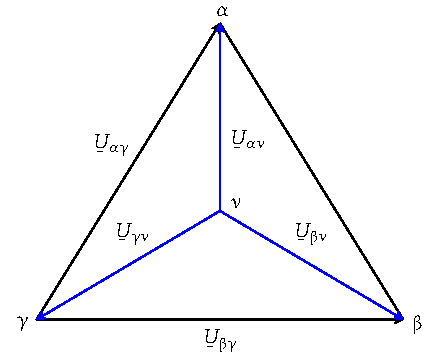
\includegraphics{Imatges/Cap-Fonaments-Potencia-Exemple.pdf}
    \end{minipage}
    \hfill
    \begin{minipage}[b][5.7cm][t]{3.8cm}
    \begin{align*}
        \cmplx{U}_{\alphaup\nuup} &= \SIpd{220}{90}{V} \\[1ex]
        \cmplx{U}_{\betaup\nuup} &= \SIpd{220}{-30}{V} \\[1ex]
        \cmplx{U}_{\gammaup\nuup} &= \SIpd{220}{210}{V} \\[1ex]
        \cmplx{U}_{\alphaup\gammaup} &= \sqrt{3}\times \SIpd{220}{60}{V} \\[1ex]
        \cmplx{U}_{\betaup\gammaup} &= \sqrt{3}\times \SIpd{220}{0}{V}
    \end{align*}
    \end{minipage}
    \hfill{}

    Els corrents $\cmplx{I}_\alphaup$, $\cmplx{I}_\betaup$ i $\cmplx{I}_\gammaup$ que
    circulen  per les tres fases s\'{o}n:
    \begin{align*}
        \cmplx{I}_\alphaup &=\frac{\cmplx{U}_{\alphaup\nuup}}{\cmplx{Z}} =
        \frac{\SIpd{220}{90}{V}}{\SIpd{22}{45}{\ohm}} =
        \SIpd{10}{45}{A}\\
        \cmplx{I}_\betaup &=\frac{\cmplx{U}_{\betaup\nuup}}{\cmplx{Z}} =
        \frac{\SIpd{220}{-30}{V}}{\SIpd{22}{45}{\ohm}} =
        \SIpd{10}{-75}{A}\\
        \cmplx{I}_\gammaup &=\frac{\cmplx{U}_{\gammaup\nuup}}{\cmplx{Z}} =
        \frac{\SIpd{220}{210}{V}}{\SIpd{22}{45}{\ohm}} =
        \SIpd{10}{165}{A}
    \end{align*}


    Per comen\c{c}ar,  utilitzarem l'equaci\'{o} \eqref{eq:s_3f_eq}, ja que tenim
    un sistema equilibrat tant pel que fa a les tensions com pel que fa a la c\`{a}rrega:
    \[
    \cmplx{S} = 3\,\cmplx{U}_{\alphaup\nuup} \,\cmplx{I}_\alphaup^* =
    3\times \SIpd{220}{90}{V} \times
    \SIpd{10}{-45}{A} = \SIpd{6600}{45}{VA}
    \]

    A continuaci\'{o},  utilitzarem l'equaci\'{o} \eqref{eq:s_3f_3fils}, ja que tenim
    un sistema d'alimentaci\'{o} de 3 fils:
    \[
    \cmplx{S} = \cmplx{U}_{\alphaup\gammaup} \,\cmplx{I}_\alphaup^*
     +  \cmplx{U}_{\betaup\gammaup} \,\cmplx{I}_\betaup^* =
    \sqrt{3}\times \SIpd{220}{60}{V} \times
    \SIpd{10}{-45}{A} + \sqrt{3}\times \SIpd{220}{0}{V}
    \times \SIpd{10}{75}{A}  = \SIpd{6600}{45}{VA}
    \]

     Finalment,  utilitzarem l'equaci\'{o} \eqref{eq:s_3f}, ja que
     sempre \'{e}s aplicable:
     \[\begin{split}
     \cmplx{S} &=  \cmplx{U}_{\alphaup\nuup} \,\cmplx{I}_\alphaup^* +
     \cmplx{U}_{\betaup\nuup} \,\cmplx{I}_\betaup^* +  \cmplx{U}_{\gammaup\nuup}\,
     \cmplx{I}_\gammaup^* =\\
     &= \SIpd{220}{90}{V}
     \times \SIpd{10}{-45}{A} + \SIpd{220}{-30}{V} \times \SIpd{10}{75}{A}
     + \SIpd{220}{210}{V} \times \SIpd{10}{-165}{A} = \SIpd{6600}{45}{VA}
     \end{split} \]

    Per acabar, veurem que tamb\'{e} es pot resoldre aquest exemple
    sense calcular els corrents; si utilitzem a l'hora les
    equacions \eqref{eq:s_3f_eq} i \eqref{eq:s_mono1}, tenim:
    \[
    \cmplx{S} = 3\,\cmplx{U}_{\alphaup\nuup} \,\cmplx{I}_\alphaup^* =
    3\,\cmplx{U}_{\alphaup\nuup}\frac{\cmplx{U}_{\alphaup\nuup}^*}{\cmplx{Z}^*} =
    3\, \frac{|\cmplx{U}_{\alphaup\nuup}|^2}{\cmplx{Z}^*} =
    3\times\frac{(\SI{220}{V})^2}{\SIpd{22}{-45}{\ohm}} =
    \SIpd{6600}{45}{VA}
    \]

    Com era d'esperar, el resultat obtingut en tots els casos
    \'{e}s id\`{e}ntic.
\end{exemple}

\subsection{Mesura de la pot\`{e}ncia}\index{pot\`{e}ncia complexa!mesura}

La pot\`{e}ncia activa es mesura amb uns aparells anomenats watt\'{\i}metres,
i la pot\`{e}ncia reactiva amb uns aparelles anomenats var\'{\i}metres.

Aquests aparells tenen dues bobines de mesura, una de voltim\`{e}trica,
la qual es connecta tal com es faria amb un volt\'{\i}metre, i una altra
d'amperim\`{e}trica, la qual es connecta tal com es faria amb un
amper\'{\i}metre; aix\'{\i} doncs, els watt\'{\i}metres i els var\'{\i}metres tenen
quatre terminals de connexi\'{o}.

La connexi\'{o} d'aquests aparells en un circuit donat, per tal de
mesurar correctament la pot\`{e}ncia, ve determinada pels dos terminals
anomenats hom\`{o}legs; un d'aquests terminals pertany a la bobina
voltim\`{e}trica i l'altre a l'amperim\`{e}trica. En els esquemes el\`{e}ctrics,
aquests dos terminals s'identifiquen mitjan\c{c}ant un punt. La connexi\'{o}
ha de fer-se de tal manera, que el corrent que va des de
l'alimentaci\'{o} cap a la c\`{a}rrega entri al watt\'{\i}metre pel terminal de
la bobina amperim\`{e}trica marcat amb el punt, i la tensi\'{o} corresponent
a aquest corrent, vagi del terminal de la bobina voltim\`{e}trica marcat
amb el punt, a l'altre terminal; el mateix \'{e}s aplicable al
var\'{\i}metre.

En la Figura \vref{pic:watt_var_mono} es pot veure la connexi\'{o} d'un
watt\'{\i}metre i d'un var\'{\i}metre en un circuit monof\`{a}sic.


\begin{center}
    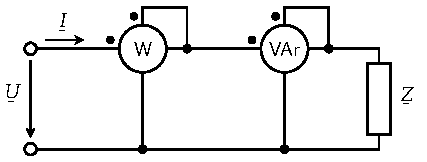
\includegraphics{Imatges/Cap-Fonaments-Mesura-Potencia-Monof.pdf}
    \captionof{figure}{Mesura de la pot\`{e}ncia en un circuit  monof\`{a}sic}
    \label{pic:watt_var_mono}
\end{center}

Les pot\`{e}ncies activa i reactiva s'obtenen de les mesures dels dos
aparells:
\begin{equation}
    P = \textsf{W} \qquad\qquad Q = \textsf{VAr}
\end{equation}

En la Figura \vref{pic:watt_var_4f} es pot veure la connexi\'{o} d'uns
watt\'{\i}metres i d'uns var\'{\i}metres en un circuit trif\`{a}sic de 4 fils,
equilibrat o desequilibrat.

\begin{center}
    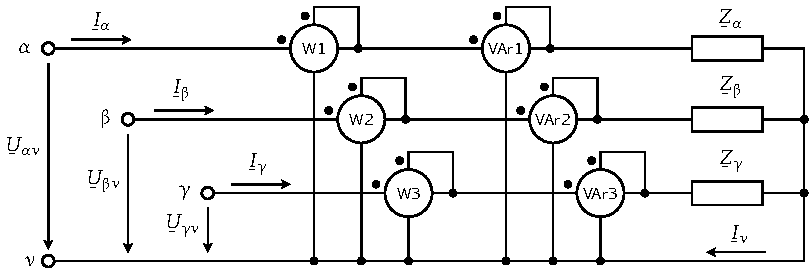
\includegraphics{Imatges/Cap-Fonaments-Mesura-Potencia-Trif-4f.pdf}
    \captionof{figure}{Mesura de la pot\`{e}ncia en un circuit  trif\`{a}sic de 4 fils}
    \label{pic:watt_var_4f}
\end{center}

Les pot\`{e}ncies activa i reactiva trif\`{a}siques s'obtenen de les mesures
dels sis aparells:
\begin{equation}
    P\ped{3F} = \textsf{W1} +  \textsf{W2} + \textsf{W3}
    \qquad\qquad Q\ped{3F} = \textsf{VAr1} +  \textsf{VAr2} + \textsf{VAr3}
\end{equation}

En la Figura \vref{pic:watt_var_3f} es pot veure la connexi\'{o} d'uns
watt\'{\i}metres i d'uns var\'{\i}metres en un circuit trif\`{a}sic de 3 fils,
equilibrat o desequilibrat.

\begin{center}
\centering
    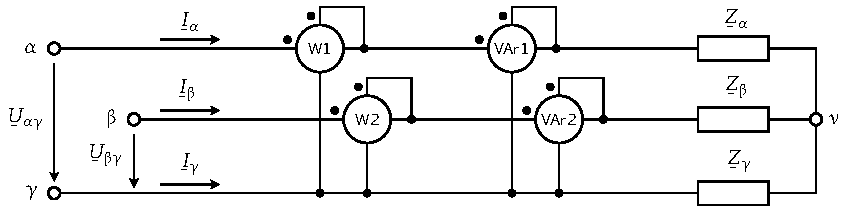
\includegraphics{Imatges/Cap-Fonaments-Mesura-Potencia-Trif-3f.pdf}
    \captionof{figure}{Mesura de la pot\`{e}ncia en un circuit  trif\`{a}sic de 3 fils}
    \label{pic:watt_var_3f}
\end{center}

Les pot\`{e}ncies activa i reactiva trif\`{a}siques s'obtenen de les mesures
dels quatre aparells:
\begin{equation}
    P\ped{3F} = \textsf{W1} +  \textsf{W2}
    \qquad\qquad Q\ped{3F} = \textsf{VAr1} +  \textsf{VAr2}
\end{equation}


\section{Components elementals d'un circuit
el\`{e}ctric}\label{sec:comp_elem}

Es presenten a continuaci\'{o} les lleis temporals que lliguen tensions,
corrents i pot\`{e}ncies, per a diversos components elementals d'un
circuit el\`{e}ctric. Es donen tamb\'{e} les relacions entre tensions i
corrents en el domini freq\"{u}encial (corrent altern sinuso\"{\i}dal, amb
$\omega=2\piup f$) i en el domini operacional (transformada de
Laplace).\index{transformada de Laplace}

Cal tenir en compte que les relacions que es donen, tan sols s\'{o}n
v\`{a}lides  quan es tenen en consideraci\'{o} els sentits assignats als
corrents i a les tensions en les figures corresponents.

\subsection{Resist\`{e}ncia} \index{resist\`{e}ncia}

\index{resist\`{e}ncia!llei temporal}Per a una resist\`{e}ncia $R$ (Figura
\vref{pic:resist}), la llei temporal entre la tensi\'{o} $u(t)$ i el
corrent $i(t)$, i la llei temporal de la pot\`{e}ncia $p(t)$ s\'{o}n:

%\vspace{-0.5mm}
\hfill
\begin{minipage}[b]{5cm}
    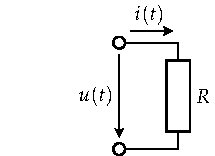
\includegraphics{Imatges/Cap-Fonaments-Resistencia.pdf}
    \captionof{figure}{Resist\`{e}ncia}
    \label{pic:resist}
\end{minipage}
\hfill
\begin{minipage}[b][3.25cm][t]{8cm}
   \begin{align}
      u(t) &= R i(t) \\  p(t) &= u(t) i(t) = R i^2(t) = \frac{u^2(t)}{R}
   \end{align}
\end{minipage}

\index{resist\`{e}ncia!domini freq\"{u}encial}En el domini freq\"{u}encial, la relaci\'{o} entre
la tensi\'{o} $\cmplx{U}$ i el corrent $\cmplx{I}$, i la relaci\'{o} entre els arguments de
la tensi\'{o} $\varphi_{\cmplx{U}}$ i del corrent $\varphi_{\cmplx{I}}$ s\'{o}n:
\begin{align}
   \cmplx{U} &= R \cmplx{I} \\ \varphi_{\cmplx{U}} &= \varphi_{\cmplx{I}}
\end{align}

\index{resist\`{e}ncia!domini operacional} En el domini operacional, la relaci\'{o} entre la tensi\'{o} $U(s)$ i el corrent $I(s)$ \'{e}s:
\begin{equation}
   U(s) = R I(s)
\end{equation}

\subsection{Capacitat} \index{capacitat}

\index{capacitat!llei temporal}Per a una capacitat $C$ (Figura
\vref{pic:capacit}), les lleis temporals entre la tensi\'{o} $u(t)$ i el
corrent $i(t)$, i la llei temporal de la pot\`{e}ncia $p(t)$ s\'{o}n:

\hfill
\begin{minipage}[b]{5cm}
    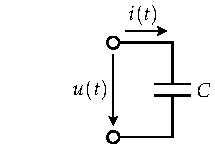
\includegraphics{Imatges/Cap-Fonaments-Capacitat.pdf}
    \captionof{figure}{Capacitat}
    \label{pic:capacit}
\end{minipage}
\hfill
\begin{minipage}[b][3.8cm][t]{8cm}
   \begin{align}
      u(t) &= u(t_0) + \frac{1}{C} \int_{t_0}^t i(t) \diff t \\
      i(t) &= C \deriv{u(t)}{t} \\
      p(t) &= u(t) i(t) = C u(t) \deriv{u(t)}{t}
   \end{align}
\end{minipage}

\index{capacitat!domini freq\"{u}encial}En el domini freq\"{u}encial, la relaci\'{o} entre la tensi\'{o} $\cmplx{U}$ i el corrent $\cmplx{I}$, i la relaci\'{o} entre els arguments de la tensi\'{o} $\varphi_{\cmplx{U}}$ i del corrent $\varphi_{\cmplx{I}}$ s\'{o}n:
\begin{align}
   \cmplx{U} &= -\ju \frac{1}{\omega C} \cmplx{I} \\
   \varphi_{\cmplx{U}} &= \varphi_{\cmplx{I}} - \frac{\piup}{2}
\end{align}

\index{capacitat!domini operacional}En el domini operacional, la relaci\'{o} entre la tensi\'{o} $U(s)$ i el corrent $I(s)$ \'{e}s:
\begin{equation}
   U(s) = \frac{1}{s C} I(s) + \frac{u(t_0)}{s}
\end{equation}


\subsection{Induct\`{a}ncia} \index{induct\`{a}ncia}

\index{induct\`{a}ncia!llei temporal}Per a una induct\`{a}ncia $L$ (Figura \vref{pic:induct}),
les lleis temporals entre la tensi\'{o} $u(t)$ i el corrent $i(t)$, i la llei temporal
de la pot\`{e}ncia $p(t)$ s\'{o}n:

\hfill
\begin{minipage}[b]{5cm}
    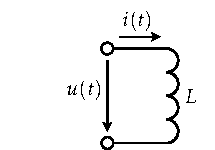
\includegraphics{Imatges/Cap-Fonaments-Inductancia.pdf}
    \captionof{figure}{Induct\`{a}ncia}
    \label{pic:induct}
\end{minipage}
\hfill
\begin{minipage}[b][3.8cm][t]{8cm}
   \begin{align}
      i(t) &= i(t_0) + \frac{1}{L} \int_{t_0}^t u(t) \diff t \\
      u(t) &= L \deriv{i(t)}{t} \\
      p(t) &= u(t) i(t) = L i(t) \deriv{i(t)}{t}
   \end{align}
\end{minipage}

\index{induct\`{a}ncia!domini freq\"{u}encial}En el domini freq\"{u}encial, la relaci\'{o} entre la tensi\'{o} $\cmplx{U}$ i el corrent $\cmplx{I}$, i la relaci\'{o} entre els arguments de la tensi\'{o} $\varphi_{\cmplx{U}}$ i del corrent $\varphi_{\cmplx{I}}$ s\'{o}n:
\begin{align}
   \cmplx{U} &= \ju \omega L \cmplx{I} \\
   \varphi_{\cmplx{U}} &= \varphi_{\cmplx{I}} + \frac{\piup}{2}
\end{align}

\index{induct\`{a}ncia!domini operacional} En el domini operacional, la relaci\'{o} entre la tensi\'{o} $U(s)$ i el corrent $I(s)$ \'{e}s:
\begin{equation}
   U(s) = s L I(s) - L i(t_0)
\end{equation}


\subsection{Acoblament magn\`{e}tic} \index{acoblament magn\`{e}tic}

\index{acoblament magn\`{e}tic!llei temporal}Per a un acoblament magn\`{e}tic $M$ entre dues
induct\`{a}ncies $L_1$ i $L_2$ (Figura \vref{pic:acobl}), les lleis temporals entre les
tensions $u_1(t)$ i $u_2(t)$ i els corrents $i_1(t)$ i $i_2(t)$,  i la llei temporal
de la pot\`{e}ncia $p(t)$ s\'{o}n:

\hfill
\begin{minipage}[b]{6cm}
   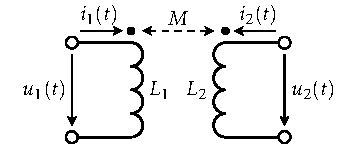
\includegraphics{Imatges/Cap-Fonaments-Acobl-Magnetic.pdf}
   \captionof{figure}{Acoblament magn\`{e}tic}
   \label{pic:acobl}
\end{minipage}
\hfill
\begin{minipage}[b][3.8cm][t]{10cm}
   \begin{align}
      u_1(t) &= L_1 \deriv{i_1(t)}{t} + M \deriv{i_2(t)}{t} \\
      u_2(t) &= L_2 \deriv{i_2(t)}{t} + M \deriv{i_1(t)}{t} \\
      p(t) &= \frac{\diff}{\diff t} \left[ \frac{1}{2} L_1 i_1^2(t) + \frac{1}{2} L_2 i_2^2(t) +
      M i_1(t) i_2(t) \right]
   \end{align}
\end{minipage}


\index{acoblament magn\`{e}tic!domini freq\"{u}encial}En el domini freq\"{u}encial, les relacions entre les tensions $\cmplx{U}_1$ i $\cmplx{U}_2$ i els corrents $\cmplx{I}_1$ i $\cmplx{I}_2$ s\'{o}n:
\begin{align}
   \cmplx{U}_1 &= \ju \omega L_1 \cmplx{I}_1 + \ju \omega M \cmplx{I}_2 \\
   \cmplx{U}_2 &= \ju \omega L_2 \cmplx{I}_2 + \ju \omega M \cmplx{I}_1
\end{align}

\index{acoblament magn\`{e}tic!domini operacional}En el domini operacional, les relacions entre les tensions $U_1(s)$  i $U_2(s)$ i els corrents $I_1(s)$ i $I_2(s)$ s\'{o}n:
\begin{align}
   U_1(s) &= s L_1 I_1(s) - L_1 i_1(t_0) + s M I_2(s) - M i_2(t_0) \\
   U_2(s) &= s L_2 I_2(s) - L_2 i_2(t_0) + s M I_1(s) - M i_1(t_0)
\end{align}

\subsection{Transformador ideal} \index{transformador ideal}

\index{transformador ideal!llei temporal}Per a un transformador
ideal de relaci\'{o} $m\!:\!1$ (Figura \vref{pic:transf}), la llei temporal
entre les tensions de primari $u_1(t)$ i de secundari $u_2(t)$, la
llei temporal entre els corrents de primari $i_1(t)$ i de secundari
$i_2(t)$, i la llei temporal de la pot\`{e}ncia $p(t)$ s\'{o}n:

\hfill
\begin{minipage}[b]{6cm}
    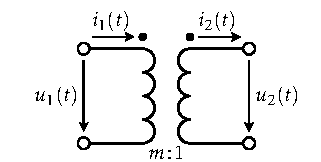
\includegraphics{Imatges/Cap-Fonaments-Trafo-Ideal.pdf}
    \captionof{figure}{Transformador ideal}
    \label{pic:transf}
\end{minipage}
\hfill
\begin{minipage}[b][3.7cm][t]{10cm}
   \begin{align}
      \frac{u_1(t)}{u_2(t)} &= m  \\
      \frac{i_2(t)}{i_1(t)} &= m \\
      p(t) &= u_1(t) i_1(t) - u_2(t) i_2(t) = 0
   \end{align}
\end{minipage}


\index{transformador ideal!domini freq\"{u}encial} En el domini
freq\"{u}encial, la relaci\'{o} entre les tensions de primari $\cmplx{U}_1$
i de secundari $\cmplx{U}_2$, la relaci\'{o} entre els corrents de
primari $\cmplx{I}_1$ i de secundari $\cmplx{I}_2$, la relaci\'{o} entre
els arguments de les tensions de primari $\varphi_{\cmplx{U}_1}$ i
de secundari $\varphi_{\cmplx{U}_2}$, i  la relaci\'{o} entre els
arguments dels corrents de primari $\varphi_{\cmplx{I}_1}$ i de
secundari $\varphi_{\cmplx{I}_2}$ s\'{o}n:
\begin{align}
   \frac{\cmplx{U}_1}{\cmplx{U}_2} &= m  \\
   \frac{\cmplx{I}_2}{\cmplx{I}_1} &= m \\
   \varphi_{\cmplx{U}_1} &= \varphi_{\cmplx{U}_2} \\
   \varphi_{\cmplx{I}_1} &= \varphi_{\cmplx{I}_2}
\end{align}

\index{transformador ideal!domini operacional} En el domini operacional, la relaci\'{o} entre les tensions de primari $U_1(s)$ i de secundari $U_2(s)$,  i la relaci\'{o} entre els corrents de primari $I_1(s)$ i de secundari $I_2(s)$ s\'{o}n:
\begin{align}
   \frac{U_1(s)}{U_2(s)} &= m  \\
   \frac{I_2(s)}{I_1(s)} &= m
\end{align}

\subsection{Bateria} \index{bateria}

\index{bateria!llei temporal}Per a una bateria $U\ped{bat}$ (Figura
\vref{pic:bat}), la llei temporal de la tensi\'{o} $u(t)$ i de la
pot\`{e}ncia $p(t)$ que subministra \'{e}s:

\hfill
\begin{minipage}[b]{5cm}
    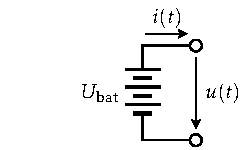
\includegraphics{Imatges/Cap-Fonaments-Bateria.pdf}
    \captionof{figure}{Bateria}
    \label{pic:bat}
\end{minipage}
\hfill
\begin{minipage}[b][3cm][t]{8cm}
   \begin{align}
      u(t) &= U\ped{bat} \\  p(t) &= U\ped{bat} i(t)
   \end{align}
\end{minipage}


El corrent $i(t)$ que circular\`{a} per la bateria, vindr\`{a} determinat
pels elements que es connectin a aquesta bateria.

\index{bateria!domini operacional} En el domini operacional, la
tensi\'{o} $U(s)$ \'{e}s:
\begin{equation}
   U(s) = \frac{U\ped{bat}}{s}
\end{equation}


\section{Circuits R-L-C}

Es presenten en aquesta secci\'{o} diversos circuits R-C i R-L, indicant les expressions temporals de les tensions i corrents que hi apareixen.

\subsection{Circuit R-C -- c\`{a}rrega en corrent continu}\index{circuit R-C!c\`{a}rrega en corrent continu}

En la figura \vref{pic:RC_serie_carrega} es representa un circuit R-C s\`{e}rie que comen\c{c}a a carregar-se a l'instant $t=0$, amb la condici\'{o} inicial: $u\ped{C}(0) = 0$, i la constant de temps: $\tau = R C$.
\begin{center}
    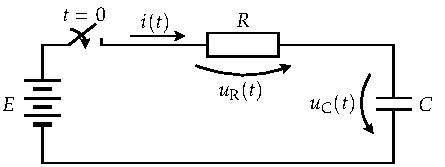
\includegraphics{Imatges/Cap-Fonaments-RC-Serie-Carrega.pdf}
    \captionof{figure}{Circuit R-C -- c\`{a}rrega en corrent continu}
    \label{pic:RC_serie_carrega}
\end{center}

Les tensions i corrents d'aquest circuit s\'{o}n:
\begin{align}
    i(t) &= \frac{E}{R}\,\eu^{-t/\tau} \\[3mm]
    u\ped{C}(t) &= E \left( 1 - \eu^{-t/\tau} \right) \\[3mm]
    u\ped{R}(t) &= E\,\eu^{-t/\tau}
\end{align}

\subsection{Circuit R-C -- desc\`{a}rrega}\index{circuit R-C!dsc\`{a}rrega}

En la figura \vref{pic:RC_serie_descarrega} es representa un circuit R-C s\`{e}rie que comen\c{c}a a descarregar-se a l'instant $t=0$, amb la condici\'{o} inicial: $u\ped{C}(0) = E$, i la constant de temps: $\tau = R C$.
\begin{center}
    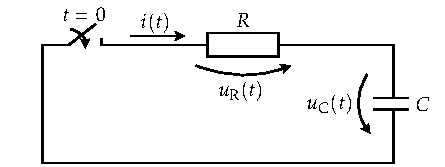
\includegraphics{Imatges/Cap-Fonaments-RC-Serie-Descarrega.pdf}
    \captionof{figure}{Circuit R-C -- desc\`{a}rrega}
    \label{pic:RC_serie_descarrega}
\end{center}

Les tensions i corrents d'aquest circuit s\'{o}n:
\begin{align}
    i(t) &= - \frac{E}{R}\,\eu^{-t/\tau} \\[3mm]
    u\ped{C}(t) &= E\,\eu^{-t/\tau} \\[3mm]
    u\ped{R}(t) &= - E\,\eu^{-t/\tau}
\end{align}

\subsection{Circuit R-L -- c\`{a}rrega en corrent continu}\index{circuit R-L!c\`{a}rrega en corrent continu}

En la figura \vref{pic:RL_serie_carrega} es representa un circuit R-L s\`{e}rie que comen\c{c}a a carregar-se a l'instant $t=0$, amb la condici\'{o} inicial: $i(0) = 0$, i la constant de temps: $\tau = L/R$.
\begin{center}
    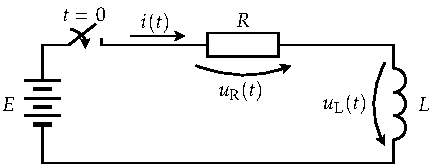
\includegraphics{Imatges/Cap-Fonaments-RL-Serie-Carrega.pdf}
    \captionof{figure}{Circuit R-L -- c\`{a}rrega en corrent continu}
    \label{pic:RL_serie_carrega}
\end{center}

Les tensions i corrents d'aquest circuit s\'{o}n:
\begin{align}
    i(t) &= \frac{E}{R}\left( 1 - \eu^{-t/\tau} \right)\\[3mm]
    u\ped{L}(t) &= E\,\eu^{-t/\tau} \\[3mm]
    u\ped{R}(t) &= E\left( 1 - \eu^{-t/\tau} \right)
\end{align}

\subsection{Circuit R-L -- desc\`{a}rrega}\index{circuit R-L!desc\`{a}rrega}

En la figura \vref{pic:RL_serie_descarrega} es representa un circuit R-L s\`{e}rie que comen\c{c}a a descarregar-se a l'instant $t=0$, amb la condici\'{o} inicial: $i(0) = I$, i la constant de temps: $\tau = L/R$.
\begin{center}
    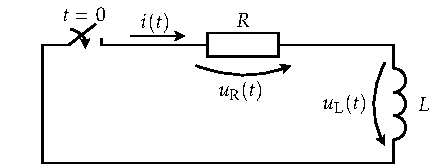
\includegraphics{Imatges/Cap-Fonaments-RL-Serie-Descarrega.pdf}
    \captionof{figure}{Circuit R-L -- desc\`{a}rrega}
    \label{pic:RL_serie_descarrega}
\end{center}

Les tensions i corrents d'aquest circuit s\'{o}n:
\begin{align}
    i(t) &= I\,\eu^{-t/\tau} \\[3mm]
    u\ped{L}(t) &= - R I\,\eu^{-t/\tau} \\[3mm]
    u\ped{R}(t) &= R I\,\eu^{-t/\tau}
\end{align}

\subsection{Circuit R-L -- curtcircuit en corrent altern}\index{circuit R-L!curtcircuit en corrent altern}

En la figura \vref{pic:RL_serie_curtcircuit} es representa un circuit R-L s\`{e}rie sotm\`{e}s a un curtcircuit en l'instant $t=0$, amb la condici\'{o} inicial: $i(0) = 0$; $u(t)$ \'{e}s una tensi\'{o} sinusoidal, on $U$ \'{e}s el seu valor efica\c{c}, $\omega = 2 \piup f$, i $\phi$ \'{e}s l'angle inicial.
\begin{center}
    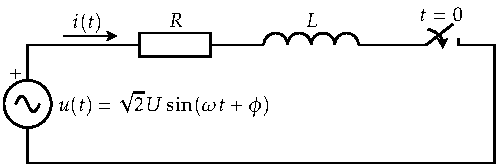
\includegraphics{Imatges/Cap-Fonaments-RL-Serie-Curtcircuit.pdf}
    \captionof{figure}{Circuit R-L -- curtcircuit en corrent altern}
    \label{pic:RL_serie_curtcircuit}
\end{center}

El corrent de curtcircuit \'{e}s:
\begin{equation}
    i(t) = i\ped{ac}(t) + i\ped{dc}(t)
    \label{eq:RL_serie_curtcircuit_icc}
\end{equation}

Amb:
\begin{subequations}
\begin{align}
    i\ped{ac}(t) &= \sqrt{2} I \sin\left(\omega t + \phi - \arctan\frac{\omega L}{R}\right) \label{eq:RL_serie_curtcircuit_iac}\\[3mm]
    i\ped{dc}(t) &= -\,\sqrt{2} I\sin\left(\phi - \arctan\frac{\omega L}{R}\right) \eu^{-t R/L}\label{eq:RL_serie_curtcircuit_idc}
\end{align}
\end{subequations}

On $I$ \'{e}s el valor efica\c{c} de $i\ped{ac}(t)$; aquest valor tamb\'{e} s'anomena valor efica\c{c} sim\`{e}tric $I\ped{sim}$, i val:
\begin{equation}
    I = I\ped{sim} =\frac{U}{\sqrt{R^2+(\omega L)^2}}
    \label{eq:RL_serie_curtcircuit_I}
\end{equation}

La component aperi\`{o}dica $i\ped{dc}(t)$ decreix exponencialment fins a fer-se zero, i finalment nom\'{e}s queda la component peri\`{o}dica $i\ped{ac}(t)$. El valor m\`{a}xim $\hat{I}$ de $i(t)$, que s'aconsegueix en els instants inicials ($t\approx 0$), dep\`{e}n del valor que pren $i\ped{dc}(0)$, i per tant dep\`{e}n del valor que apareix en l'equaci\'{o} \eqref{eq:RL_serie_curtcircuit_idc}: $\sin\left(\phi - \arctan\frac{\omega L}{R}\right)$; en circuits for\c{c}a inductius ($\omega L\gg R$), aquest valor \'{e}s m\`{a}xim quan $\phi \approx 0$, i $\hat{I}$ pren el valor te\`{o}ric:
\begin{equation}
    \hat{I} = 2 \sqrt{2} I
\end{equation}


En aquest mateix cas (circuit for\c{c}a inductiu i $\phi \approx 0$), tamb\'{e} \'{e}s m\`{a}xim el valor efica\c{c} inicial de $i(t)$, tamb\'{e} anomenat valor efica\c{c} asim\`{e}tric $I\ped{asim}$,  i val:
\begin{equation}
    I\ped{asim} = \sqrt{i\ped{dc}^2(0) + I^2} = \sqrt{\left(\sqrt{2}I\right)^2 + I^2} = \sqrt{3} I
\end{equation}

Pel mateix raonament, el valor m\'{\i}nim de $i(t)$ en circuits for\c{c}a inductius, s'aconsegueix quan $\phi \approx \pm\frac{\pi}{2}$. En Aquest cas $i\ped{dc}(t)$ es fa zero des de l'inici, i nom\'{e}s queda la component alterna $i\ped{ac}(t)$.

\begin{exemple}[Curtcircuit en un circuit R-L]
    Es tracta de calcular el corrent de curtcircuit que circula pel circuit de la Figura \vref{pic:RL_serie_curtcircuit}, amb els valors seg\"{u}ents: $U=\SI{400}{V}, f=\SI{50}{Hz}, \phi=\SI{0}{rad}, R=\SI{9e-4}{\ohm}, L=\SI{5e-5}{H}$.

    Primer calculem els valors:
    \begin{align*}
        \omega &= 2\pi f = 2\times\pi\times\SI{50}{Hz} = \SI{314,1593}{rad/s} \\[3mm]
        \arctan\frac{\omega L}{R} &= \arctan\frac{\SI{314,1593}{rad/s}\times\SI{5e-5}{H}}{\SI{9e-4}{\ohm}} =
        \SI{1,5136}{rad} \\[3mm]
        \sin\left(\phi - \arctan\frac{\omega L}{R}\right) &= \sin(\SI{0}{rad} - \SI{1,5136}{rad})= \num{-0,9984}
    \end{align*}

    A continuaci\'{o}, utilitzant l'equaci\'{o} \eqref{eq:RL_serie_curtcircuit_I}, tenim:
    \[
        I=\frac{\SI{400}{V}}{\sqrt{\left(\SI{9e-4}{\ohm}\right)^2+\left(\SI{314,1593}{rad/s}\times \SI{5e-5}{H}\right)^2}} =
        \SI{25423,0955}{A}
    \]

    Finalment, a partir d'aquests valors i de les equacions \eqref{eq:RL_serie_curtcircuit_icc}, \eqref{eq:RL_serie_curtcircuit_iac} i \eqref{eq:RL_serie_curtcircuit_idc}, tenim:
    \[
        i(t) = \num{35953,6865}\sin(\num{314,1593}\,t-\num{1,5136}) + \num{35894,8169}\,\eu^{-18 t}
    \]

    Per acabar, representem a continuaci\'{o} la funci\'{o} $i(t)$:
    \begin{center}
        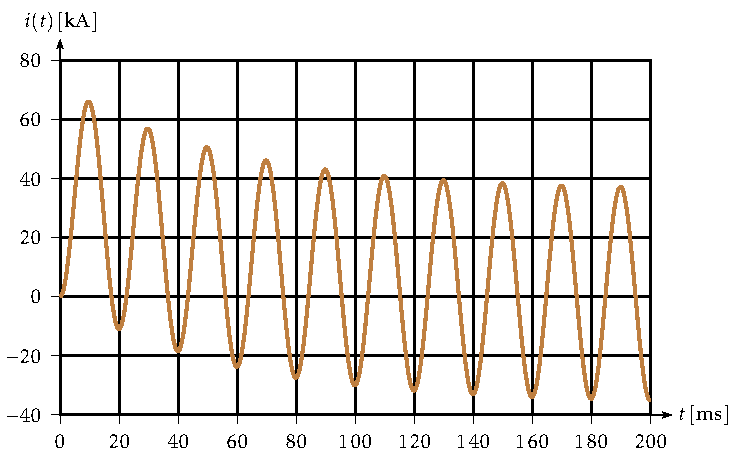
\includegraphics{Imatges/Cap-Fonaments-Exemple-R-L.pdf}
    \end{center}
\end{exemple} 